\documentclass[./examen.tex]{subfiles}
\begin{document}
\begin{center}
\makebox[\textwidth]{Nombre y Apellido:\enspace\hrulefill}
\end{center}
\begin{questions}
\question Resolver los siguientes problemas.
\begin{parts}
 \part[20] Un conductor que se desplaza con una velocidad $v=30\frac{m}{s}$ perpendicular a un campo magnético de inducción $B=36,\hat{6}T$, sabiendo que la longitud es $l=20cm$. Calcular la fuerza electro motriz $f.e.m$ inducida en el conductor en volts $V$.
 
 \begin{center}
 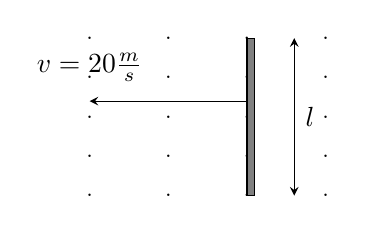
\begin{tikzpicture}
 \draw [stealth-stealth](0.6,0) -- (0.6,2);
 \node at (0.8,1) {$l$};
 \draw [fill=gray](0,0) rectangle (0.1,2);
 \draw [-stealth] (0,1.2) -- (-2,1.2)  node[label={$v=20\frac{m}{s}$}]{};
 \foreach \y in {0,1,2,...,4}{
    \foreach \x in {-4,-2,...,2}{
    \node at (\x/2,\y/2) {\footnotesize $.$};
    }
}
 \end{tikzpicture}
 \end{center}
 
 \part[2] \begin{tabular}{ p{12cm} p{3cm} }
El anillo cilíndrico de la figura de sección $S=5cm^2$ está construído de chapa magnética, se desea un flujo de $\Phi =75000Mx$. Calcular la inducción magnética en el núcleo, longitud de la línea media y amperios -vuelta necesarios.& \begin{center}
    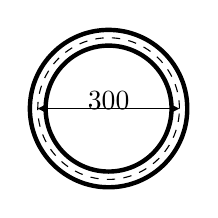
\begin{tikzpicture}[scale=0.01]
    \draw [dashed, thin] (0,0) circle [radius=90];
    \draw [ultra thick] (0,0) circle [radius=100];
    \draw [ultra thick] (0,0) circle [radius=80];
    \draw [stealth-stealth] (-90,0)--(90,0);
    \draw (0,10) node[]{300};
    \end{tikzpicture}
    \end{center}
  \end{tabular}
  \part[2] ¿Qué intensidad $I$ debe circular por un conductor que tiene $l=10cm$ de longitud dentro de un campo magnético de inducción $B=1400Gs$, si está cortando perpendicularmente a las líneas de fuerza del campo para que se ejerza sobre el conductor $F=0,5N$?
  \part[2] Un solenoide de $N=2000$ espiras, longitud de $l=50cm$, $\varnothing=4cm$ y núcleo de madera el cual tiene arrollado sobre él una bobina de $N=1500$ espiras. Calcular la f.e.m. inducida en la bobina cuando se anula en $\Delta t=0,1s$. La corriente es de $I=10A$ 
 \end{parts}
 \question Explicar la regla de la mano izquierda, dar 2 ejemplos.
 
 
 
 \end{questions}
 \end{document}